\section{Adding Lattices to Bloom}
\label{sec:impl}

\begin{figure}[t]
\begin{scriptsize}
\begin{lstlisting}
class ShortestPaths
  include Bud

  state do
    table :link, [:from, :to, :c]
    table :path, [:from, :to, :next_hop] => [:c]
    table :min_cost, [:from, :to] => [:c]
  end

  bloom do
    path <= link {|l| [l.from, l.to, l.to, MinLattice.new(l.c)]}
    path <= (link*path).pairs(:to => :from) do |l,p|
      [l.from, p.to, l.to, p.c + l.c]
    end
    min_cost <= path {|p| [p.from, p.to, p.c]}
  end
end
\end{lstlisting}
\end{scriptsize}
\caption{A \lang program to compute the all-pairs shortest paths of a
  graph.}
\label{fig:lattice-spaths}
\end{figure}

% Outline:
% * design philosophy, sign posting
% * introduce lattice values
% * introduce lattice wrappers
% * introduce morphisms
% * discuss example program
% * discuss integration features
% * implementation notes

% XXX: need intro paragraph

% is this the right place for this?
When designing \lang, we decided to extend Bloom to include support for
lattices rather than building a new language from scratch. Hence, \lang is
backward compatible with Bloom, and was implemented with relatively minor
changes to the Bud runtime. This design decision also required that we consider
rules written over lattices should interoperate with rules that use traditional
Bloom relations; we added several \lang features to ease this interoperability,
which we describe in Section~\ref{sec:bloom-interop}.

\subsection{Lattice classes and elements}
In \lang, each lattice has an associated Ruby class, which we call the
\emph{lattice class}. An instance of this class is called a \emph{lattice
  element}. A lattice element represents a single point in the lattice---i.e., an
element of the poset associated with the lattice.

A lattice class is a normal Ruby class that meets a certain API contract. Every
lattice class inherit from the builtin \texttt{Bud::Lattice} class, and
must also define two methods:
\begin{itemize}
\item \texttt{initialize(i)}: given a Ruby object \emph{i}, this method
  constructs a new lattice element that ``wraps'' \emph{i} (\texttt{initialize}
  is just the normal Ruby syntax for defining a constructor). By convention, the
  Ruby value wrapped by a lattice element is assigned to a Ruby member variable
  \texttt{@v}. If $i$ is the null reference, this method returns the least
  element of the lattice.

\item \texttt{merge(e)}: given a lattice element \emph{e}, this method returns the
  lattice element that is the least upper bound of $\{e, \textit{self}\}$. This method must
  satisfy the algebraic properties summarized in Section~\ref{sec:found-defn}---in
  particular, it must be commutative, associative, and idempotent. Note that
  \emph{e} must have the same class as \emph{self}.
\end{itemize}
Lattice elements are \emph{immutable} (e.g., \texttt{merge} functions should
construct a new lattice element rather than modifying one of their inputs
in-place). Efficient lattice implementations may \emph{share structure} on merge
operations, as is common practice for immutable data structures in functional
programming languages~\cite{Okasaki1999}. % XXX: maybe not the right place for this

\subsection{Morphisms and OPMs}
As described in Section~\ref{sec:foundation}, morphisms allow complex programs
to be created via the composition of multiple lattices. In \lang, a morphism is
akin to a Ruby method that satisfies the algebraic properties summarized in
Section~\ref{sec:found-defn}.

\subsection{Program analysis}

\begin{figure}[t]
\begin{scriptsize}
\begin{lstlisting}
class Bud::SetLattice < Bud::Lattice
  wrapper_name :lset

  def initialize(x=[])
    # Reject invalid input (elided)
    @v = x.uniq # Remove duplicates from input
  end

  def merge(i)
    self.class.new(@v | i.reveal)
  end

  morph :intersect do |i|
    self.class.new(@v & i.reveal)
  end

  morph :pro do |&blk|
    @v.map(&blk)
  end

  ord_map :size do
    Bud::MaxLattice.new(@v.size)
  end
end
\end{lstlisting}
\end{scriptsize}
\caption{The implementation of the \texttt{lset} lattice in Ruby.}
\label{fig:lattice-set}
\end{figure}

\subsection{Integration with set-oriented logic}
\label{sec:bloom-interop}

\lang provides two features to ease integration of lattice-based code with
traditional Bloom programs that manipulate set-oriented collections.

\subsubsection{Implicit fold}
% XXX: this ignores the fact that Bloom collections consist of sets of tuples,
% whereas implicit fold works for sets of singleton values
% XXX: refer to shortest paths program as practical example
This feature enables set-oriented collections to be more easily used as input to
lattices. If a \lang rule has a set-oriented collection on the rhs and a lattice
on the lhs, the lattice merge function is used to ``fold over'' the elements of
the collection. That is, each element of the collection is converted to a
lattice element (via the appropriate lattice constructor); then the set of
lattice elements are merged together (via repeated application of the
\texttt{merge} method). In our experience, this is typically the behavior
intended by the user.

\subsubsection{Collections with embedded lattice values}
It would be convenient to allow lattice elements to be stored as attributes of
tuples that appear in set-oriented Bloom collections. Furthermore, Bloom
provides several facilities (e.g., network communication, persistent storage,
module interfaces) as collections with special semantics; it would be
unfortunate if a redundant set of facilities would be necessary to support
lattice-based code. A simple solution would be to extract the underlying Ruby
value from the lattice element (e.g., using the \texttt{reveal} method), and
then store that value as a tuple attribute in a set-oriented
collection. Unfortunately, that would introduce needless non-monotonicity into
the program.

Storing lattice elements as attributes of tuples in set-oriented collections
introduces several challenges. Consider a simple \lang rule that derives tuples
with a lattice element as an attribute value:
\begin{verbatim}
    t1 <= t2 {|t| [t.x, lat_foo]}
\end{verbatim}
where \texttt{t1} and \texttt{t2} are Bloom relations and \texttt{lat\_foo}
identifies a lattice; suppose that the first column of \texttt{t1} is the
relation's key. The value associated with \texttt{lat\_foo} can change over the
course of the fixpoint computation (specifically, it can grow ``upward''
according to the lattice's partial order). Implemented naively, this might
result in multiple \texttt{t1} tuples with different values for the second
attribute, which would violate \texttt{t1}'s key (the first column of
\texttt{t1} would not functionally determine a single value for the second
column).

This problem could be avoided by requiring that lattice elements embedded into
Bloom collections be computed exactly before the rule that performs the
embedding is evaluated. This would effectively stratify the program according to
lattice embedding rules, which would disallow cycles through lattice
embeddings~\cite{Apt1988}. This would reject intuitively reasonable programs; it
also seems unsatisfying to require stratification of monotonic programs.

% Clarify this
Instead, \lang allows rules to produce multiple tuples that differ only in their
embedded lattice values. During the course of the fixpoint computation, those
values are merged together using the appropriate lattice merge function. This is
safe because any functions that might be computed over the embedded lattice
value must be monotonic. Nevertheless, this solution is somewhat
counterintuitive, because tuples in Datalog relations are traditionally
immutable: once a fact is known to be true, its value remains the
same.\footnote{Bloom facts can be deleted, but this is an explicit non-monotonic
  operation that can only occur between timesteps. Conceptually, Bloom models
  update as the retraction of the previous version of a fact and the insertion
  of a new fact~\cite{dedalus}.}
% Should we note that we might add an option to disable this behavior for
% particular attributes?

\subsection{Implementation}

\subsubsection{Lattice wrappers}
A \emph{lattice wrapper} manages the mapping from identifier names to lattice
elements.

\begin{table*}[t]
\begin{tabular}{|l|l|l|l|l|}
\hline
\textbf{Name} & \textbf{Description} & \textbf{Merge} & \textbf{Morphisms} & \textbf{OPMs}\\
\hline
\texttt{lbool} & Boolean lattice (false $\to$ true) & & \texttt{when\_true} & \\
\texttt{lmax} & Max over an ordered domain & &\texttt{gt},
\texttt{gt\_eq}, \texttt{+}, \texttt{-} & \\
\texttt{lmin} & Min over an ordered domain & &\texttt{lt}, \texttt{lt\_eq},
\texttt{+}, \texttt{-} & \\
\texttt{lset} & Set of values & & \texttt{intersect}, \texttt{product},
\texttt{project} & \texttt{size} \\
\texttt{lpset} & Set of non-negative numbers & &
\texttt{intersect}, \texttt{product}, \texttt{project}& \texttt{size}, \texttt{sum} \\
\texttt{lbag} & Multiset of values & & \texttt{intersect},
\texttt{project}, \texttt{mult(k)}, \texttt{+} & \texttt{size}\\
\texttt{lmap} & Map from key to lattice values & &
\texttt{intersect}, \texttt{project}, \texttt{at(k)}, \texttt{key?(k)} & \texttt{size}\\
\hline
\end{tabular}
\caption{The builtin lattice types in \lang.}
\label{tbl:builtin-lattices}
\end{table*}

\subsection{Performance study}
\begin{figure}[t]
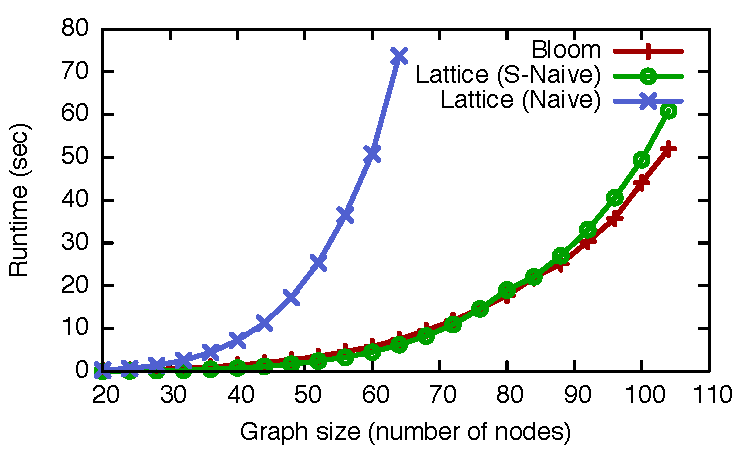
\includegraphics[width=\linewidth]{fig/sn_perf}
\caption{Performance comparison of three different methods for computing the
  transitive closure of a graph.}
\label{fig:tc-perf-graph}
\end{figure}

To validate the effectiveness of semi-naive evaluation for \lang programs, we
wrote two versions of a program to compute the transitive closure of a directed
acyclic graph. One version was written in Bloom and used traditional
set-oriented collections. The other version was written in \lang and used
morphisms over the \texttt{lset} lattice. For the \lang version, we ran the
program both with and without semi-naive evaluation enabled. We ran the programs
on synthetic graphs of various sizes---in a graph with $n$ nodes, each node had
approximately $\log_2 n$ outgoing edges. We ran the experiment on a late 2010
MacBook Air with a 2.13 Ghz Intel Core 2 Duo processor and 4GB of RAM, running
Mac OS X 10.7.3 and Ruby 1.8.7-p352. We ran each program variant five times on
each graph and report the mean wall-clock time.

Figure~\ref{fig:tc-perf-graph} shows how the runtime of each program varied with
the size of the graph. Note that we only report results for the naive \lang
strategy on small input sizes because this variant exhibited exponential
performance. The poor performance of naive evaluation is not surprising: after
deriving all paths of length $n$, naive evaluation will then rederive all those
paths at every subsequent ``step'' of the fixpoint computation. In contrast,
after computing length $n$ paths, a semi-naive strategy will only generate
length $n+1$ paths in the next step. Bloom and semi-naive \lang achieve similar
results. These results suggest that our implementation of semi-naive evaluation
for \lang is effective and performs comparably with semi-naive evaluation for a
traditional Datalog system.
